\documentclass[12pt,a4paper]{article}
\usepackage{graphicx}
\usepackage{listings}
\usepackage{color}
\usepackage{hyperref}
\usepackage{geometry}
\usepackage{float}
\usepackage{caption}
\usepackage{subcaption}
\usepackage{tabularx}
\usepackage{booktabs}
\usepackage{svg}

\geometry{margin=1in}

% Code listing style
\definecolor{codegreen}{rgb}{0,0.6,0}
\definecolor{codegray}{rgb}{0.5,0.5,0.5}
\definecolor{codepurple}{rgb}{0.58,0,0.82}
\definecolor{backcolour}{rgb}{0.95,0.95,0.92}

\lstdefinestyle{mystyle}{
    backgroundcolor=\color{backcolour},   
    commentstyle=\color{codegreen},
    keywordstyle=\color{magenta},
    numberstyle=\tiny\color{codegray},
    stringstyle=\color{codepurple},
    basicstyle=\ttfamily\footnotesize,
    breakatwhitespace=false,         
    breaklines=true,                 
    captionpos=b,                    
    keepspaces=true,                 
    numbers=left,                    
    numbersep=5pt,                  
    showspaces=false,                
    showstringspaces=false,
    showtabs=false,                  
    tabsize=2
}
\lstset{style=mystyle}

\title{CS256 Class Project Report: FPGA Tetris}

\author{
    Mohammad Alkhalifah \\
    \texttt{mohammad.alkhalifah@kaust.edu.sa}
    \and
    Mustafa Albahrani\thanks{Contributed to the project implementation; however, this report is an individual submission by Mohammad Alkhalifah} \\
    \texttt{mustafa.albahrani@kaust.edu.sa}
}

\date{\today}



\begin{document}

\maketitle
\newpage

\tableofcontents
\newpage

\section{Introduction}
The objective of this class project was to implement a fully functional Tetris game on an FPGA verification board. The project utilizes SystemVerilog to describe the hardware logic required for generating VGA video signals, processing user input via a PS/2 keyboard, and maintaining the complex game state.

The system is designed to interface with standard peripherals: a VGA monitor for display and a keyboard for control. The implementation demonstrates key digital design concepts such as finite state machines (FSMs), clock domain crossing (CDC), protocol handling (PS/2), video timing generation, and pipelined rendering.

\section{VGA Signaling and Timing Generation}
VGA (Video Graphics Array) is an analog video transmission standard that requires precise timing signals to control the electron beam in a CRT monitor (or the pixel scanning in modern LCDs).

\subsection{Protocol Overview}
The video signal consists of three color channels (Red, Green, Blue) and two synchronization pulses:
\begin{enumerate}
    \item \textbf{Horizontal Sync (HS)}: Signals the end of a line and controls the horizontal retrace.
    \item \textbf{Vertical Sync (VS)}: Signals the end of a frame and controls the vertical retrace.
\end{enumerate}

To achieve the target resolution of $1280 \times 800$ (scaled to simpler timings) or standard $640 \times 480$, our system operates with a pixel clock of approximately 83.46 MHz.

\subsection{Circuit Implementation}
We implemented the timing logic in the \texttt{vga\_out} module. Two counters, \texttt{hcount} and \texttt{vcount}, track the scanning beam's position.
The horizontal counter \texttt{hcount} increments on every pixel clock, resetting after reaching \texttt{H\_MAX} (1679). The vertical counter \texttt{vcount} increments whenever \texttt{hcount} completes a line.

The synchronization pulses are generated by comparing these counters against specific thresholds defined in the README specifications:

\begin{lstlisting}[language=Verilog, caption=VGA Sync Logic in vga\_out.sv]
// README SPEC: hsync 0 when hcount 0-135 (Active Low)
assign hsync = ~(hcount <= H_SYNC_END); // H_SYNC_END = 135

// README SPEC: vsync 1 when vcount 0-2 (Active High)
assign vsync = (vcount <= V_SYNC_END);  // V_SYNC_END = 2
\end{lstlisting}

\subsection{Determining Pixel Coordinates}
To draw objects, we must know the coordinate of the pixel currently being rendered. The raw counters include "blanking" intervals (front/back porch) where no video is sent. We calculate \texttt{curr\_x} and \texttt{curr\_y} relative to the \textit{visible} area only.

The \texttt{active\_area} signal is high only when the counters are within the visible window.

\begin{lstlisting}[language=Verilog, caption=Active Area and Coordinate Calculation]
// Active Area Definition
assign active_area = (hcount >= H_VIS_START && hcount <= H_VIS_END) &&
                     (vcount >= V_VIS_START && vcount <= V_VIS_END);

// Coordinate Calculation (Relative to Top-Left of Screen)
// Output coordinates relative to active area
always_comb begin
    if (active_area) begin
        curr_x = hcount - H_VIS_START; // Offset by 336
        curr_y = vcount - V_VIS_START; // Offset by 27
    end else begin
        curr_x = 0; curr_y = 0;
    end
end
\end{lstlisting}

As visualized in Figure \ref{fig:vga_sch}, the synthesized schematic confirms this logic. The large counter blocks (seen as accumulators in the center) correspond to \texttt{hcount} and \texttt{vcount}, while the comparators on the right generate the sync pulses based on the parameters defined in \texttt{GLOBAL.sv}. This hardware implementation ensures cycle-accurate timing compliant with the VESA standard.

\begin{figure}[H]
    \centering
    \includegraphics[width=1.0\textwidth]{Schematic/VGA_inst_pics/full_vga.png}
    \caption{Synthesized Schematic of the `vga\_out` module showing counters and sync comparators.}
    \label{fig:vga_sch}
\end{figure}

\section{Module Architecture}
The system serves as a complex hierarchy of SystemVerilog modules. Below is a definition of the key components and their roles in the design:

\vspace{0.3cm}
\noindent
\begin{tabularx}{\textwidth}{@{} l X @{}}
\toprule
\textbf{Module} & \textbf{Description} \\
\midrule
\texttt{game\_top} & The top-level wrapper. It generates all system clocks (using MMCM or dividers), handles the global reset, and instantiates the IO drivers (VGA, PS/2). \\[0.5em]

\texttt{vga\_out} & The video timing levelgenerator. It produces the \texttt{hsync}, \texttt{vsync}, and \texttt{active\_area} signals required for the $1280 \times 800$ display standard. \\[0.5em]

\texttt{game\_control} & The core logic hub. It contains the main FSM that governs game flow (spawning, gravity, line clearing) and maintains the board state array. \\[0.5em]

\texttt{draw\_tetris} & The rendering engine. It takes the game state and current pixel coordinate to output an RGB color, leveraging sprites and using a multi-stage pipeline. \\[0.5em]

\texttt{input\_manager} & The input processor. It implements Delayed Auto Shift (DAS) to make controls feel responsive, converting raw key presses into game commands. \\[0.5em]

\texttt{check\_valid} & A combinational logic block that checks if a proposed piece position collides with walls or existing blocks. \\[0.5em]

\texttt{ghost\_calc} & A helper module that calculates the "shadow" position of the piece by projecting it downwards until a collision occurs. \\
\bottomrule
\end{tabularx}

\section{Design Description and Drawing Logic}

\subsection{Drawing Strategy: Pipelined Renderer}
Drawing Objects on the screen is performed by the \texttt{draw\_tetris} module. Unlike software rendering which clears a buffer and redraws, hardware rendering must decide the color of \textit{the specific pixel being clocked out right now}.

To handle the complex decision making within a single pixel clock cycle ($<$12ns), the design uses a pipelined approach shown in Figure \ref{fig:draw_pipeline}.

\begin{enumerate}
    \item \textbf{Stage 1: Region Detection (Fig \ref{fig:draw_pipeline}a).} Logic comparators classify the current \texttt{curr\_x/y} pixel into regions: Board, Next Piece, Score, or Border. This reduces the problem space for the next stages.
    \item \textbf{Stage 2: Data Access.} Based on the region, the system fetches data from the game board RAM or character ROM.
    \item \textbf{Stage 3: Sprite Output (Fig \ref{fig:draw_pipeline}b).} The retrieved block ID is used to address the Sprite ROM. The schematic shows the multiplexing logic that selects the final pixel color based on the sprite data and piece type (Cyan, Purple, etc.).
\end{enumerate}

\subsection{4-Stage Pipeline Details}
The logic checks the grid coordinates derived from \texttt{curr\_x/y}. If the pixel corresponds to a non-empty cell in the \texttt{display.data} array, we assign a color index.

\begin{lstlisting}[language=Verilog, caption=Grid Drawing Logic (draw\_tetris.sv)]
// Calculate Grid Indices
s1_grid_col <= (curr_x - GRID_X_START) / BLOCK_SIZE;
s1_grid_row <= (curr_y - GRID_Y_START) / BLOCK_SIZE;

// Check if block exists
if (display.data[s1_grid_row + 2][s1_grid_col].data != `TETROMINO_EMPTY) begin
    s2_cell_color_idx <= display.data[s1_grid_row + 2][s1_grid_col].data + 1;
end
\end{lstlisting}

This logic ensures that as the beam scans across the screen, it "picks up" the color of the Tetris block at that location.

\subsection{Clock Architecture}
The system utilizes a complex clocking scheme to balance performance and protocol requirements. Five distinct clock domains are generated:
\begin{itemize}
    \item \textbf{100 MHz}: Main system clock and 7-segment display driver.
    \item \textbf{83.46 MHz}: Pixel clock for 1280x800 VGA timing.
    \item \textbf{50 MHz}: PS/2 clock for reliable keyboard sampling (2x oversampling of max PS/2 frequency).
    \item \textbf{25 MHz}: Game Logic clock. The FSM runs here to allow simple single-cycle logic without timing violations relative to the fast pixel clock.
    \item \textbf{60 Hz}: Game Tick. Generated from the 25 MHz clock to drive gravity and animation updates.
\end{itemize}
Figure \ref{fig:clock_arch} shows the synthesized clock generation circuit and the CDC synchronizers used to safely transfer signals between domains.

\begin{figure}[H]
    \centering
    \begin{subfigure}[b]{0.48\textwidth}
        \centering
        \includegraphics[width=\textwidth]{Schematic/game_top_pics/clk_section.png}
        \caption{Clock Generation Circuit}
    \end{subfigure}
    \hfill
    \begin{subfigure}[b]{0.48\textwidth}
        \centering
        \includegraphics[width=\textwidth]{Schematic/game_top_pics/cdc_section.png}
        \caption{CDC Synchronizers}
    \end{subfigure}
    \caption{Clock Architecture and Domain Crossing Logic.}
    \label{fig:clock_arch}
\end{figure}

\subsection{Input Processing}
The input system ensures that player controls are fluid. As shown in Figure \ref{fig:input_das}, the implementation relies on dedicated counters for the "Delayed Auto Shift" (DAS) mechanism.
The counters (`timer\_left` and `timer\_right` visible in the schematic) increment whilst a key is held. Once they cross a threshold (DAS\_DELAY), the system generates rapid movement pulses. This hardware-based timing ensures that the repeat rate is independent of the frame rate or game logic load.

\begin{figure}[H]
    \centering
    \begin{subfigure}[b]{0.48\textwidth}
        \centering
        \includegraphics[width=\textwidth]{Schematic/input_mgr_pics/left0.png}
        \caption{Left DAS Counter}
    \end{subfigure}
    \hfill
    \begin{subfigure}[b]{0.48\textwidth}
        \centering
        \includegraphics[width=\textwidth]{Schematic/input_mgr_pics/right0.png}
        \caption{Right DAS Counter}
    \end{subfigure}
    \caption{Input Manager DAS Logic for Left/Right Movement.}
    \label{fig:input_das}
\end{figure}

\subsubsection{PS/2 Keyboard Protocol}
The project supports full keyboard input via the PS/2 protocol. The \texttt{PS2Receiver} module implements the low-level deserialization, sampling the PS/2 clock and data lines to extract 11-bit frames (1 start, 8 data, 1 parity, 1 stop). These raw scan codes are then decoded by \texttt{ps2\_keyboard}, which handles:
\begin{itemize}
    \item \textbf{Make/Break Detection}: A \texttt{0xF0} prefix indicates a key release.
    \item \textbf{Extended Codes}: A \texttt{0xE0} prefix is used for arrow keys and special keys.
\end{itemize}
The decoded key events are synchronized to the game clock domain using a 3-stage synchronizer chain to avoid metastability.

\subsection{Game Logic}
The core logic resides in `game\_control`. It works in tandem with specialized sub-modules:

\subsubsection{Randomizer (7-Bag System)}
To ensure fair gameplay, we implemented a \textbf{7-Bag Randomizer} in `generate\_tetromino.sv`. Instead of pure random selection, the system generates a "bag" of all 7 pieces and draws from it until empty, then regenerates. This guarantees that a player will never go more than 13 moves without seeing a specific piece (e.g., the 'I' bar).

\subsubsection{Rotation System (SRS)}
The project implements the \textbf{Super Rotation System (SRS)} standards. The `rotate\_tetromino` module handles:
\begin{itemize}
    \item Basic 90-degree matrix rotation.
    \item \textbf{Wall Kicks}: If a rotation would cause a collision, the system tries alternative offsets (up, left, right) derived from standard look-up tables. This allows players to rotate pieces even in tight spaces.
\end{itemize}

\subsubsection{Scoring and Level Progression}
The score is calculated using classic NES Tetris rules, scaled by the current level:
\begin{itemize}
    \item Single: 40 $\times$ (Level + 1)
    \item Double: 100 $\times$ (Level + 1)
    \item Triple: 300 $\times$ (Level + 1)
    \item Tetris (4 lines): 1200 $\times$ (Level + 1)
\end{itemize}
The level increases every 10 lines cleared, which in turn speeds up the gravity (drop timer decreases). This is implemented in \texttt{game\_control.sv} using a lookup table for \texttt{drop\_speed\_frames}.

\subsubsection{T-Spin Detection}
Modern Tetris rewards advanced techniques like the T-Spin, where the T-piece rotates into a tight spot. The \texttt{spin\_detector} module checks if the piece is "immobile" (3 of 4 corners occupied) immediately after a rotation. If true and lines are cleared, bonus points are awarded. Figure \ref{fig:tspin_example} illustrates a typical T-Spin scenario.

\begin{figure}[H]
    \centering
    \includegraphics[width=0.8\textwidth]{tspin-example.jpg}
    \caption{Example of a T-Spin: The T-piece rotates into a slot where it is immobile.}                                                                                                                                                                            
    \label{fig:tspin_example}
\end{figure}
\subsubsection{Finite State Machine (FSM)}
The complex behavior of the game is governed by a central FSM in \texttt{game\_control.sv}. Figure \ref{fig:fsm} shows the state transitions between the 15 states, including the main loops for input handling (`IDLE`), piece manipulation (`MOVE`/`ROTATE`), and gravity (`DOWN`). The key states are summarized in Table \ref{tab:fsm_states}.

\begin{figure}[H]
    \centering
    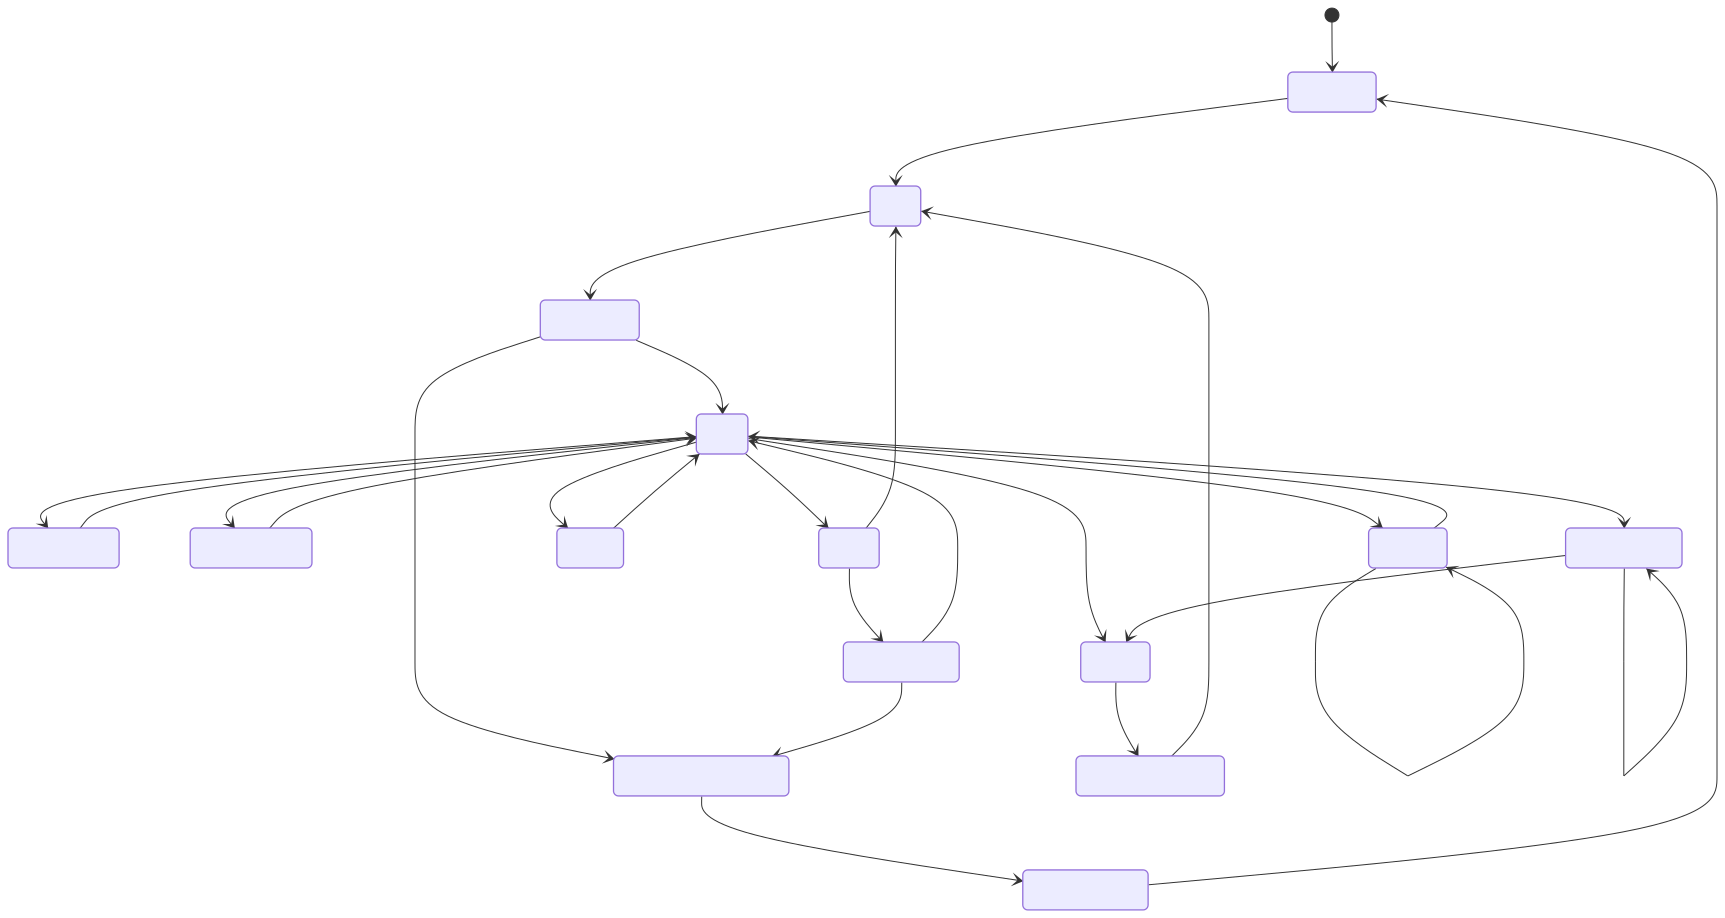
\includegraphics[width=1\textwidth]{fsm_diagram.png}
    \caption{Game Control FSM Diagram showing major state transitions.}
    \label{fig:fsm}
\end{figure}

\begin{table}[H]
    \centering
    \begin{tabular}{|l|l|}
    \hline
    \textbf{State} & \textbf{Description} \\ \hline
    \texttt{GEN} & Spawns a new tetromino from the randomizer. \\ \hline
    \texttt{IDLE} & Waits for user input (Left, Right, Rotate) or gravity timer. \\ \hline
    \texttt{MOVE\_*} & Updates x-coordinate. Checks collision; reverts if invalid. \\ \hline
    \texttt{ROTATE} & Tries standard rotation. If invalid, attempts Wall Kicks (SRS). \\ \hline
    \texttt{DOWN} & Moves piece down. If blocked, locks piece and goes to CLEAN. \\ \hline
    \texttt{CLEAN} & Scans for full rows, removes them, and shifts grid down. \\ \hline
    \texttt{HOLD} & Swaps current piece with held piece (if allowed). \\ \hline
    \texttt{GAME\_OVER} & Halts game until reset command is received. \\ \hline
    \end{tabular}
    \caption{Description of Main FSM States in \texttt{game\_control}.}
    \label{tab:fsm_states}
\end{table}

\subsubsection{Ghost Piece}
The `ghost\_calc` module continuously calculates where the current piece would land if dropped instantly. This "Ghost Piece" is rendered semi-transparently to aid player accuracy. Figure \ref{fig:drop_rot} shows the hardware logic for the drop and rotate operations.

\begin{figure}[H]
    \centering
    \includegraphics[width=0.8\textwidth]{Schematic/game_inst/drop_rot.png}
    \caption{Logic for piece manipulation (Drop and Rotate).}
    \label{fig:drop_rot}
\end{figure}

\subsection{Display Logic}
The display logic is decoupled from the game state update rate.
\begin{itemize}
    \item \textbf{CDC for Display}: The game state (field, current piece position) is transferred from the game domain to the pixel domain at the start of each frame (VSync) to ensure a tear-free image.
    \item \textbf{Rendering}: `draw\_tetris` calculates the color of the current pixel.
    \item \textbf{Sprites}: A ROM-based sprite system (`block\_sprite`) adds a beveled 3D look to the blocks. The sprites are stored as grayscale and tinted dynamically based on the piece type (e.g., Cyan for 'I', Purple for 'T').
\end{itemize}

\subsubsection{Sprite System Details}
The \texttt{block\_sprite} module stores a 16x16 pixel grayscale texture in ROM. Each pixel is a 12-bit value representing a brightness level. During rendering:
\begin{enumerate}
    \item The current pixel's position within a 32x32 block is calculated (using \texttt{curr\_x \% 32}).
    \item This address is sent to the sprite ROM, which returns a brightness value.
    \item The brightness is multiplied by a per-piece color (e.g., Cyan for I, Purple for T) to produce the final RGB output.
\end{enumerate}
This allows a single sprite texture to be reused for all 7 piece types, saving ROM space.

\begin{figure}[H]
    \centering
    \begin{subfigure}[b]{1.0\textwidth}
        \centering
        \includegraphics[width=\textwidth]{Schematic/draw_inst_pics/region_detectoin.png}
        \caption{Region Detection Logic (Stage 1)}
    \end{subfigure}
    \\
    \begin{subfigure}[b]{1.0\textwidth}
        \centering
        \includegraphics[width=\textwidth]{Schematic/draw_inst_pics/sprit_output.png}
        \caption{Sprite Output Logic (Stage 3)}
    \end{subfigure}
    \caption{Rendering Pipeline Implementation: Region detection determines the active object, while the sprite pipeline fetches pixel data.}
    \label{fig:draw_pipeline}
\end{figure}

\subsection{Game Logic Integration}
The game state is managed by the \texttt{game\_control} module. It handles:
\begin{itemize}
    \item \textbf{Gravity}: A counter generates a "tick" (approx 60Hz) to move pieces down.
    \item \textbf{Collisions}: The \texttt{check\_valid} module predicts next positions to prevent overlapping.
    \item \textbf{Ghost Piece}: We calculate where the piece would land if dropped instantly and render it semi-transparently.
\end{itemize}

\section{Testing and Verification}
We developed a comprehensive suite of testbenches to verify individual modules before integration. All simulations were run in Vivado XSim.

\subsection{Testbench Summary}
Table \ref{tab:tb_summary} lists the key testbenches and their verification targets.

\begin{table}[H]
    \centering
    \begin{tabular}{|l|l|c|}
    \hline
    \textbf{Testbench} & \textbf{Module Under Test} & \textbf{Result} \\ \hline
    \texttt{tb\_game\_control} & Core FSM (IDLE, MOVE, CLEAN) & 9/9 PASS \\ \hline
    \texttt{tb\_input\_manager} & DAS, One-Shot logic & 17/17 PASS \\ \hline
    \texttt{tb\_rotate\_tetromino} & CW/CCW rotation matrix & 4/4 PASS \\ \hline
    \texttt{tb\_hold\_feature} & Hold swap, lockout & 9/9 PASS \\ \hline
    \texttt{tb\_generate\_tetromino} & 7-Bag randomizer & 13/13 PASS \\ \hline
    \texttt{tb\_vga\_out} & Sync pulse timing & Visual Pass \\ \hline
    \end{tabular}
    \caption{Summary of Testbenches and Results.}
    \label{tab:tb_summary}
\end{table}

\subsection{Input Manager Test (\texttt{tb\_input\_manager})}
This testbench verifies \textbf{DAS} (Delayed Auto Shift) and \textbf{One-Shot} behavior. The log confirms that the rotation commands only fire once per key press, and the DAS repeat only triggers after a delay.

\begin{verbatim}
Test 1: Rotate CW One-Shot
  PASS: Rotate CW Triggered on press
  PASS: Rotate CW Pulse Ended after one cycle
  PASS: Rotate CW did not re-trigger while holding

Test 4: Left DAS (Delayed Auto Shift)
  PASS: Left Initial Move on press
  PASS: No trigger during DAS delay (15 frames)
  PASS: Left DAS Auto-Repeat Triggered
\end{verbatim}

\subsection{Rotation Test (\texttt{tb\_rotate\_tetromino})}
This testbench checks the basic matrix rotation (CW and CCW), ensuring the rotation index wraps correctly (e.g., $3 \rightarrow 0$ for CW).

\begin{verbatim}
Test 1: CW 0 -> 1
PASS: CW rotation 0 -> 1
Test 2: CW wrap 3 -> 0
PASS: CW rotation 3 -> 0
Test 3: CCW 0 -> 3
PASS: CCW rotation 0 -> 3
\end{verbatim}

\subsection{Hold Feature Test (\texttt{tb\_hold\_feature})}
This tests the swap-and-lockout mechanic. It verifies that after one hold, the player cannot hold again until a new piece has been placed.

\begin{verbatim}
Test 2: First Hold (Empty -> Store)
  Current piece before hold: J (1)
  After hold: curr=O, hold=J, hold_used=1
  PASS: First piece stored in hold

Test 3: Hold Lockout (Cannot Hold Twice Per Piece)
  Attempting second hold while hold_used=1...
  PASS: Lockout prevented second hold
\end{verbatim}

\subsection{Randomizer Test (\texttt{tb\_generate\_tetromino})}
Verified that the 7-Bag randomizer produces valid piece indices on sequential requests.

\begin{verbatim}
=== Test 2: Sequential Generation ===
PASS: Piece 0 - Valid index: 2
PASS: Piece 1 - Valid index: 2
...
PASS: Piece 9 - Valid index: 3
\end{verbatim}

\subsection{VGA Timing Test (\texttt{tb\_vga\_out})}
We ran a basic simulation over several frame periods to visually confirm that \texttt{hsync} and \texttt{vsync} pulsed at the expected intervals. The waveform was inspected to ensure \texttt{active\_area} was asserted only within the visible pixel range.

\subsection{Hardware Validation}
On the physical FPGA board (Nexys A7), we verified:
\begin{itemize}
    \item \textbf{Visual Output}: The Tetris grid is centered, block colors match type (Cyan I, Purple T), and the ghost piece renders correctly.
    \item \textbf{Input Response}: The DAS feels responsive, similar to official Tetris games.
    \item \textbf{Gameplay}: Full games were played through including line clears, reaching max level, game over, and reset functionality.
\end{itemize}


\section{Code Quality}
The code employs robust design patterns:
\begin{itemize}
    \item \textbf{Parameters}: All constants (screen size, sync pulses) are defined as \texttt{localparam} or in \texttt{GLOBAL.sv}.
    \item \textbf{Separation of Logic and Display}: The game logic updates the state array, while the display logic purely reads it. This prevents "tearing" and logic bugs.
    \item \textbf{Naming Conventions}: Signals are clearly named (\texttt{t\_next}, \texttt{s1\_curr\_x} for Stage 1 pipeline).
\end{itemize}

\section{Reflection}
\textit{(To be filled by student)}
I enjoyed working on the video timing generation as it provided a concrete understanding of how digital signals translate to visual information. One challenge was handling the clock domain crossing between the slow game logic (60Hz tick) and the fast pixel clock, which resulted in some initial visual glitches that were solved by synchronizing state updates to VSync. In the future, I would improve the project by adding audio output and more advanced scoring animations.

\newpage
\appendix
\section{Appendix: Verilog Code}

\subsection{Top Level}
\lstinputlisting[language=Verilog]{game_top.sv}

\subsection{Display Modules}
\lstinputlisting[language=Verilog]{src/display/vga_out.sv}
\lstinputlisting[language=Verilog]{src/display/draw_tetris.sv}

\subsection{Logic Modules}
\lstinputlisting[language=Verilog]{src/logic/game_control.sv}
\lstinputlisting[language=Verilog]{src/logic/check_valid.sv}
\lstinputlisting[language=Verilog]{src/logic/clean_field.sv}

\subsection{Input Modules}
\lstinputlisting[language=Verilog]{src/input/ps2_keyboard.sv}
\lstinputlisting[language=Verilog]{src/input/input_manager.sv}

\end{document}
